\documentclass[../pflichtenheft.tex]{subfiles}

\begin{document}

%Title and table of content
\maketitle
\tableofcontents

\clearpage

\section{Praeambel}
	Wer gerne beim Joggen Musik hört, der kennt es: Ein neuer Song beginnt, der einen die Anstrengung vergessen lässt. Dabei versucht man seinen Schrittrhythmus unterbewusst an den Beat des Songs anzupassen. Gelingt einem das, so motiviert es einen nur noch mehr, immer weiter zu laufen.

	\begin{center}
		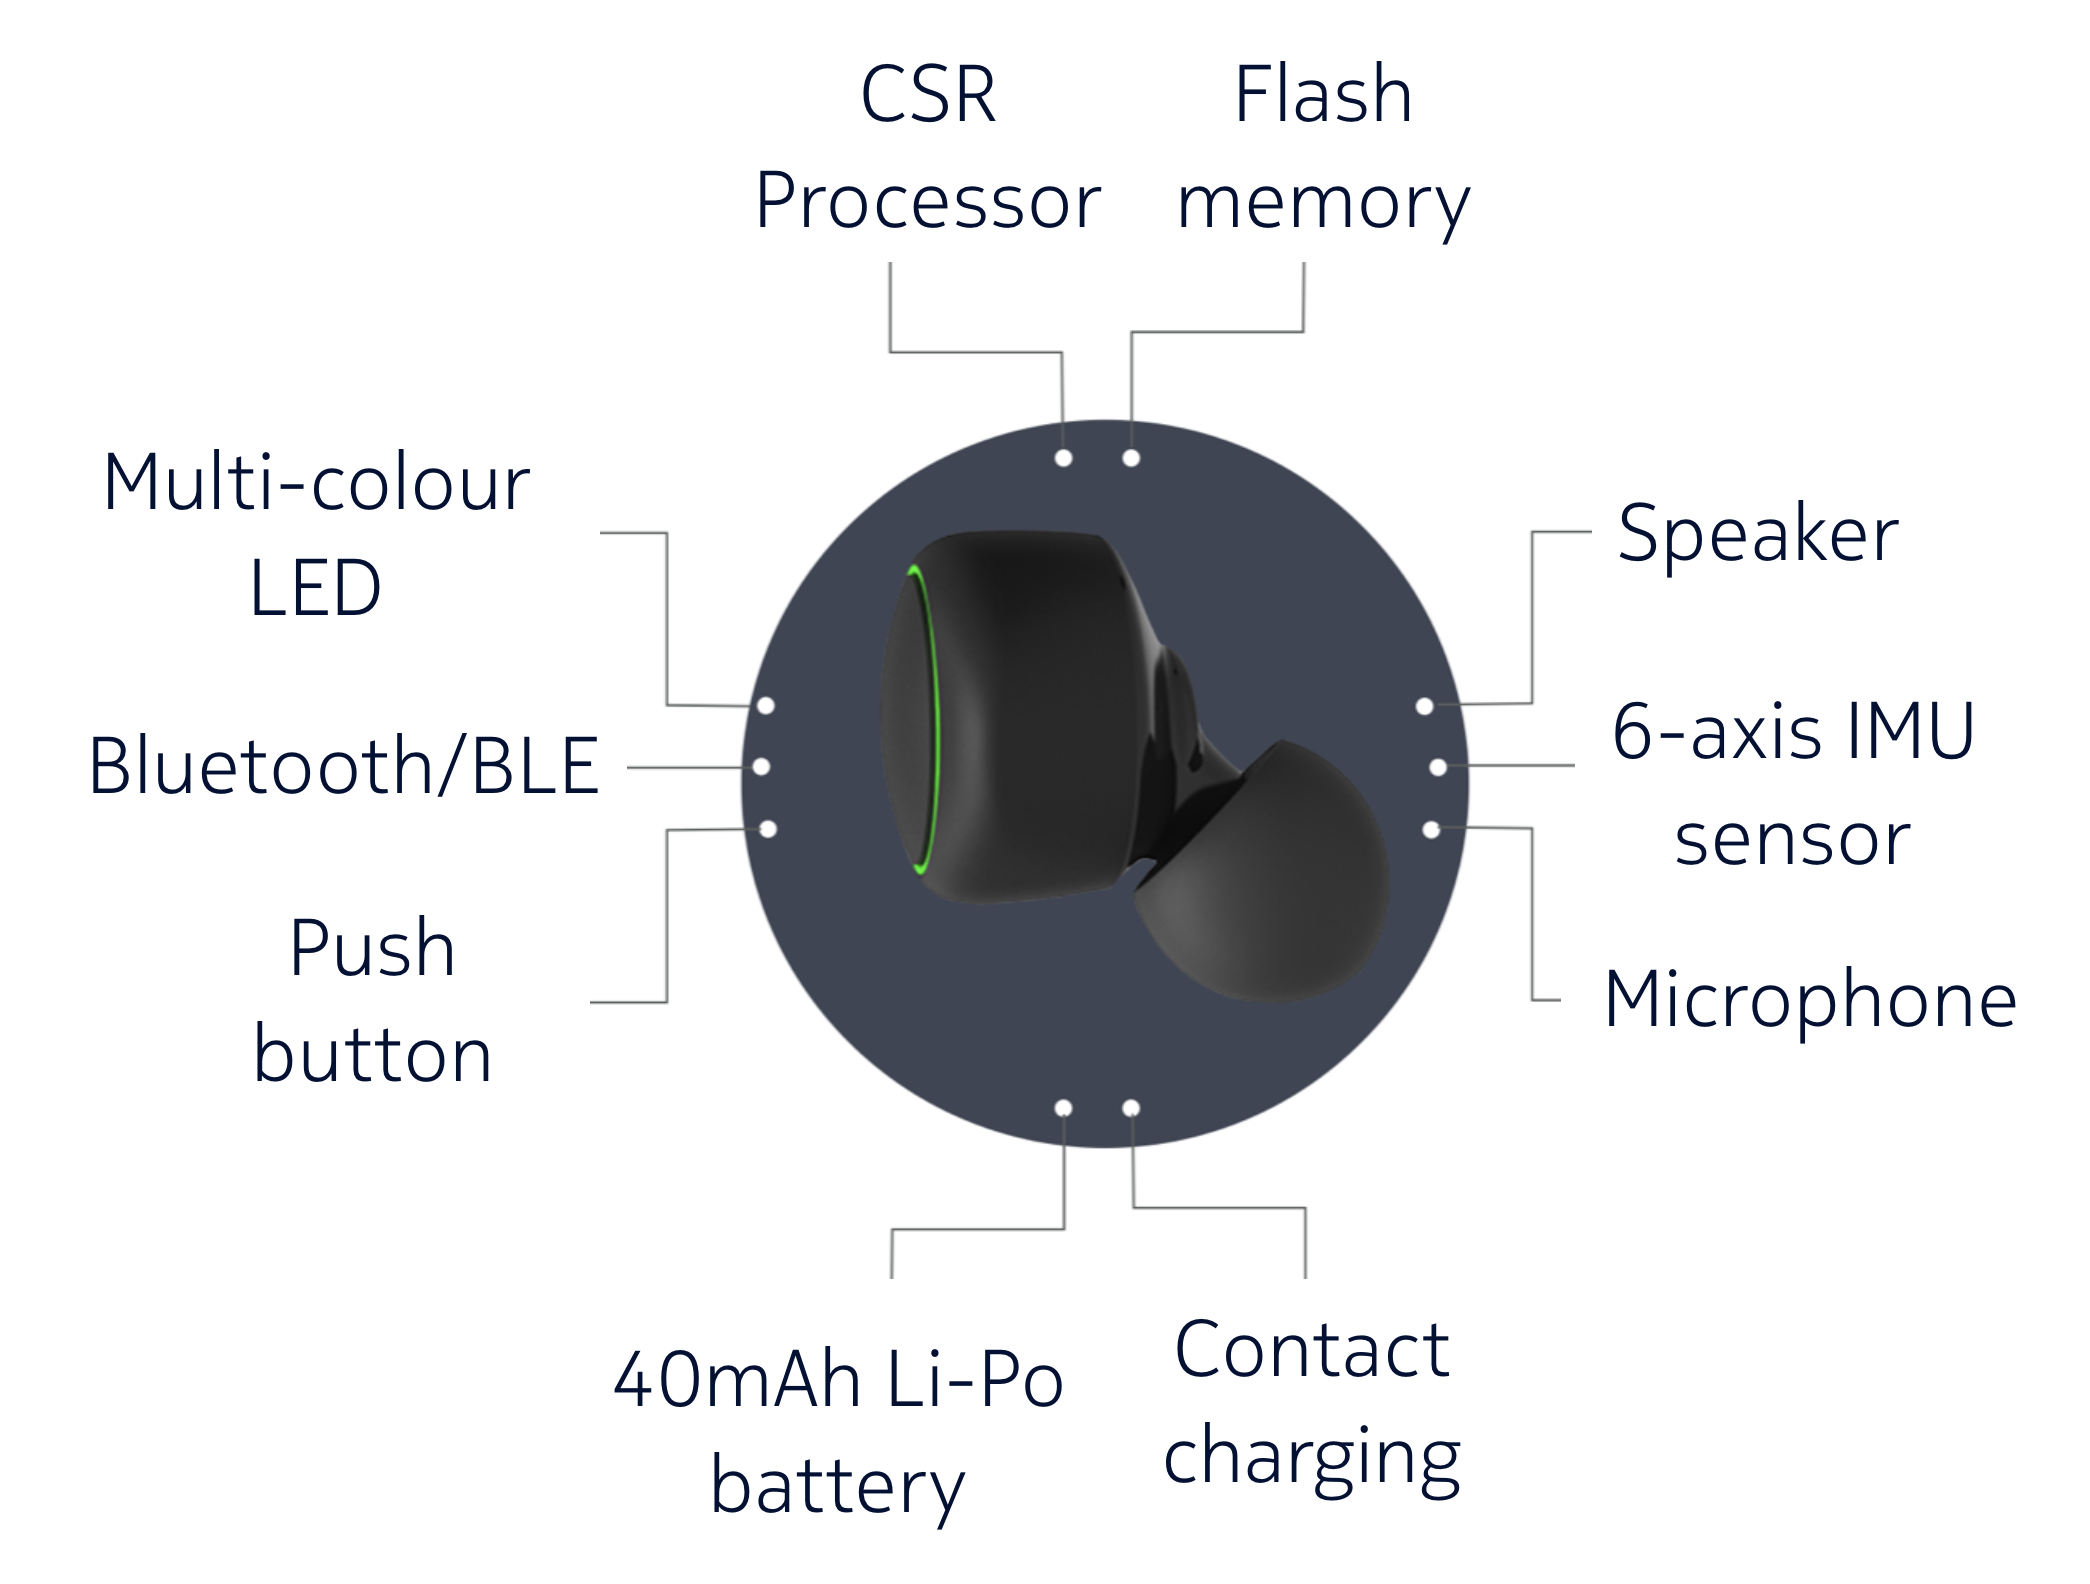
\includegraphics[page=1,width=350pt,keepaspectratio]{../graphics/Praeambel/esense.png}
		\textit{Spezifikation der \Gls{earable}-Plattform \quote{\gls{esense}}}
	\end{center}

	Das Ziel dieses Projekts ist es deshalb, eine minimalistisch gestaltete und intuitiv nutzbare \Gls{app} für mobile \Gls{device}e zu entwickeln, welche die Schrittfrequenz des \Gls{user}s berechnen kann, um passend dazu Songs abzuspielen.
	Die Schritterkennung wird dabei mit der \Gls{earable}-Plattform \quote{\gls{esense}} realisiert. Diese besitzt eingebaute Bewegungs-\Gls{sensor}en, deren Daten dann über \Gls{bt} an das \Gls{device} übertragen und dort von der \Gls{app} ausgewertet werden.

\end{document}
